\documentclass[11pt,a4paper]{article}
\usepackage[utf8]{inputenc}
\usepackage[T1]{fontenc}
\usepackage{lmodern}
\usepackage{textcomp}
\usepackage{amsmath,amssymb}
\usepackage{graphicx}
\usepackage{booktabs}
\usepackage{longtable}
\usepackage{array}
\usepackage{listings}
\usepackage{xcolor}
\usepackage[margin=1in]{geometry}
\usepackage{float}
\usepackage[hidelinks,breaklinks]{hyperref}
\usepackage{microtype}
\setlength{\parskip}{4pt}
\lstset{basicstyle=\ttfamily\scriptsize,breaklines=true,breakatwhitespace=false,
  postbreak=\mbox{\textcolor{gray}{$\hookrightarrow$}\space},frame=single,
  framerule=0.3pt,rulecolor=\color{gray!60},columns=fullflexible,keepspaces=true,
  showstringspaces=false,numbers=none,xleftmargin=4pt,xrightmargin=4pt,
  literate={\_}{{\_}}1}
\graphicspath{{figures/}}
\providecommand{\tightlist}{}
\title{The Thermal Pure Higgsino at 1.0--1.2 TeV: Relic Mass, Direct-Detection Limits and the LZ 248 keV Event}
\author{HEP-Genesis-Agent session record \\ \small Project: ramp-research-higgsino-dd}
\date{2026-10-22}
\begin{document}
\maketitle
\noindent\textit{\small This document is an AI-generated account of an interactive session with the HEP-Genesis agent. Its text was written by a language model strictly from the session record; figures and numbers come only from tool results obtained during the session. The supplementary material and the transcript, generated alongside, document exactly what ran. Verify independently before use.}
\vspace{1em}

\begin{abstract}
We report a tool-assisted literature and computational assessment of the pure-higgsino thermal relic target. Three questions were addressed: the mass at which a pure higgsino reproduces the Planck 2018 abundance, how it compares with LZ and XENONnT, and how it fares under the 2026 interpretations of a single LZ nuclear-recoil candidate as higgsino inelastic scattering. The work proceeded in two research passes. In the first pass no relic-density tool was connected. The one published pure-higgsino point found, $\Omega h^2=0.127$ (perturbative) and $0.126$ (Sommerfeld) from arXiv:1411.6930, was rescaled as $m^2$ to give a thermal mass of about 1.14 TeV. This rescaling has low confidence and rests on a mass assignment inferred from context.

In the second pass an inelastic-DM tool server was available. Its perturbative freeze-out calculation gives $\Omega h^2=0.0731$, 0.0898, 0.1083, 0.1285 and 0.1503 at $m_\chi=0.9$--1.3 TeV and crosses 0.120 at $\approx1159$ GeV. This crossing reflects the tool's built-in normalisation rather than an independent calculation. An independent Sommerfeld plus bound-state value of $1.08\pm0.02$ TeV was read from arXiv:2205.04486; it is marked contested.

For elastic scattering, Chen and Hill (arXiv:1912.07795) place the pure-higgsino signal below neutrino backgrounds at TeV masses. The LZ 2024 limit is $2.2\times10^{-48}$ cm$^2$ at 40 GeV. Its value at 1.1 TeV was not read; a linear extrapolation of about $6\times10^{-47}$ cm$^2$ is an estimate only. The XENONnT limit at 1 TeV was not obtained.

For inelastic scattering, the tool's truncated standard halo ($v_{\rm esc}+v_E=776$ km/s) gives zero LZ events for every splitting $\delta\geq380$ keV at 1.0--1.2 TeV. LZ-compatible counts appear only at $\delta\approx350$ keV, below the solar-neutrino exclusions at 475 keV and 557 keV reported in the literature. Analytic kinematics show that the published preferred region of 481--519 keV requires Earth-frame speeds of roughly 920--980 km/s at $E_R=248$ keV. A thermal pure higgsino is therefore not excluded by elastic xenon limits, and its inelastic interpretation of the LZ event depends entirely on the halo's high-velocity tail.
\end{abstract}

\section{Introduction}

The user posed one question, repeated three times over the session. It had three parts: survey recent arXiv work on the higgsino thermal relic target at 1.0--1.2 TeV; use the inelastic-DM tools to compute the relic density at several masses; and compare with LZ/XENONnT sensitivities and the Planck abundance to determine where the higgsino sits relative to current limits.

The session answered this in two research passes. The first pass ran when no relic-density or inelastic-DM compute tool was connected, so the relic density had to be reconstructed from the literature. It produced a report, after which the question was repeated. The second pass ran with an inelastic-DM tool server available. That pass also took up a strand of recent literature the first pass had not reached: a single LZ nuclear-recoil candidate at $E_R=248$ keV, interpreted in 2026 papers as inelastic higgsino scattering, and the solar-neutrino and gamma-ray limits on that interpretation.

The scope therefore covers four topics:
\begin{itemize}
\item the thermal relic mass;
\item elastic spin-independent (SI) scattering against xenon limits;
\item inelastic $Z$-mediated scattering and the kinematic reach in the neutral splitting $\delta$;
\item the halo dependence of the LZ-event interpretation.
\end{itemize}

\section{Methods}

\paragraph{Literature tools.} Literature work used abstract search (local and arXiv API), metadata lookup and full-text download. Chunked reading of the extracted PDF text was used to obtain numbers. A citation tool validated verbatim quotes against the extracted text before adding entries to a bibliography file. Figures were requested from papers through an HTML figure extractor. A shared research board recorded findings with confidence levels, open questions and dead ends, and a critic reviewed plans, waves and reports. All execution was local; the dispatch tool reported ``local execution''.

\paragraph{First pass.} The catalog contained only statistics, histogram, test-job and literature tools, and \texttt{list\_input\_files} returned an empty set. No $\Omega h^2$ was therefore computed in this pass. Every relic value is either read from a paper or obtained by labelled rescaling of a published point.

\paragraph{Second pass.} An inelastic-DM server (\texttt{serve-idm.sh}) was available, with tools \texttt{compute\_relic\_density}, \texttt{predict\_recoil}, \texttt{check\_all\_constraints}, \texttt{scan\_mass\_splitting}, \texttt{predict\_annual\_modulation}, \texttt{plot\_recoil\_spectrum} and \texttt{plot\_constraint\_summary}. Its self-description lists Lewin \& Smith (rate formula), Kolb \& Turner (freeze-out), Arkani-Hamed et al.\ (hep-ph/0601041, higgsino relic) and Planck 2018 as references.

The relic tool performs perturbative freeze-out with the following settings:
\begin{itemize}
\item a higgsino default $\langle\sigma v\rangle = 2.5\times10^{-26}\,{\rm cm^3\,s^{-1}}\times(1100\,{\rm GeV}/m_\chi)^2$;
\item $x_f\approx24.4$--24.8 and $g_*=86.25$;
\item a Planck reference of $0.12\pm0.0012$.
\end{itemize}

The recoil tools assume the following:
\begin{itemize}
\item a xenon target and per-nucleon cross section $\sigma_n\simeq7.43\times10^{-39}$ cm$^2$;
\item a standard halo with a hard cutoff at $v_{\rm esc}+v_E=776$ km/s;
\item the LZ extended nuclear-recoil exposure of 2.84 tonne-years.
\end{itemize}
No tool exposes halo parameters.

\paragraph{Hand kinematics.} The analysis used $m_N=131\times0.9315$ GeV $=122.0$ GeV, reduced mass $\mu$, and the inelastic threshold
\begin{equation}
v_{\min}(E_R)=\frac{1}{\sqrt{2m_NE_R}}\left(\frac{m_NE_R}{\mu}+\delta\right),\qquad
\delta_{\max}(E_R)=v_{\max}\sqrt{2m_NE_R}-\frac{m_NE_R}{\mu},\qquad
\delta_{\max}^{\rm abs}=\tfrac12\mu v_{\max}^2 .
\end{equation}
These follow the minimum-velocity relation cited from Appendix A of arXiv:2609.09830. The supplement holds the full tool-call log.

\section{Results}

\subsection{First pass: literature-only relic density and limits}

\paragraph{Planck target.} The Planck 2018 abstract (arXiv:1807.06209) was read to state ``A combined analysis gives dark matter density $\Omega_ch^2 = 0.120\pm0.001$'' at 68\% confidence. A later attempt to validate the string ``0.120 \textbackslash pm 0.001'' through the citation tool failed because the PDF math was garbled. The value was read, but the quote is not in the bibliography file.

\paragraph{Published pure-higgsino relic point.} Beneke, Hellmann and Ruiz-Femen\'ia (arXiv:1411.6930, Sec.~3) give two sets of numbers:
\begin{itemize}
\item a pure-higgsino model with sfermions and heavy Higgses decoupled: $\Omega h^2=0.127$ (perturbative) and $0.126$ (Sommerfeld, with off-diagonal rates);
\item the higgsino-like pMSSM point 1627006 (higgsino fraction 0.98, $\Delta m_+=1.8$ GeV, $\Delta m_0=9.5$ GeV): 0.108 perturbative and 0.100 with Sommerfeld, an 8\% reduction.
\end{itemize}
The net pure-higgsino Sommerfeld effect is below 1\%. The paper attributes this to enhancement in the neutral channels cancelling suppression in the $\chi^0\chi^\pm$ channels. Assigning $m_\chi=1172.31$ GeV, the pMSSM point's mass, to the pure-higgsino numbers was inferred from context, not stated. This finding is contested on the board.


\begin{figure}[H]
\centering
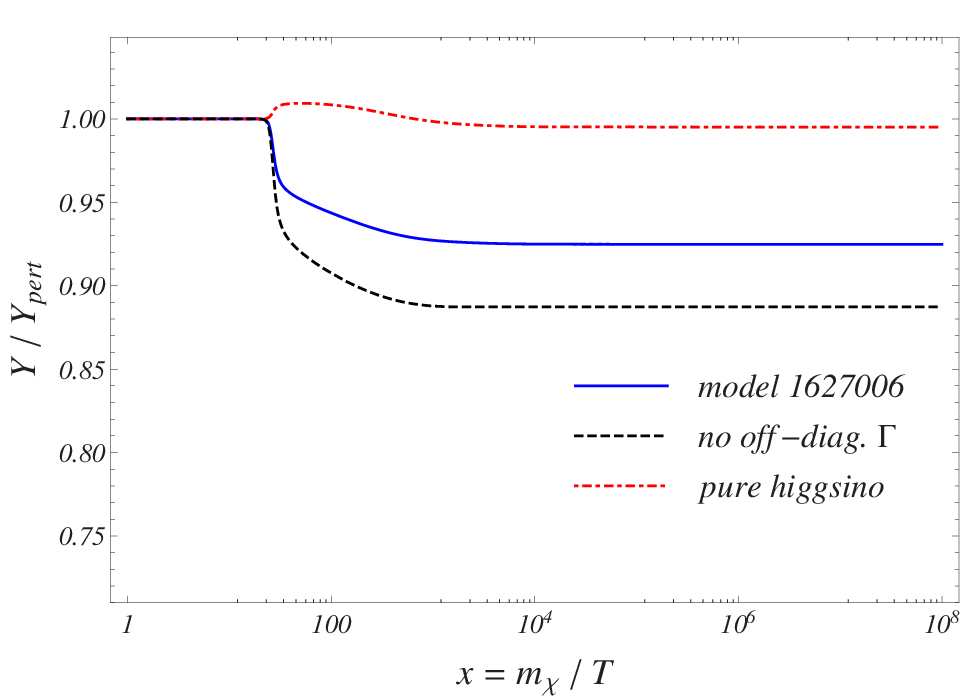
\includegraphics[width=0.85\textwidth,height=0.6\textheight,keepaspectratio]{fig-6.png}
\caption{Figure 7: The ratio of the yields Y/Y\_\{\textbackslash{}text\{pert\}\}, where Y is calculated including Sommerfeld enhancements on the annihilation rates and Y\_\{\textbackslash{}text\{pert\}\} uses purely perturbative rates. The solid (blue) line corresponds to the calculation within the pMSSM Snowmass model 1627006 with higgsino-like \textbackslash{}chi\textasciicircum{}\{0\}\_\{1\}, that includes off-diagonal annihilation rates. The dashed (black) line gives the same result but with neglected off-diagonal rates. The dot-dashed curve is the result (with off-diagonal rates) obtained for the pure-higgsino model. [arXiv:1411.6930] Reproduced from arXiv:1411.6930 (extracted with \texttt{get\_paper\_figures}).}
\label{fig:6}
\end{figure}



Figure~\ref{fig:6} reproduces Fig.~7 of arXiv:1411.6930. It shows the yield ratio $Y/Y_{\rm pert}$ for three cases: the pMSSM higgsino-like model with and without off-diagonal rates, and the pure-higgsino model with off-diagonal rates. It indicates the size of the Sommerfeld correction rather than an $\Omega h^2(m)$ curve. Its relevance is that, for the pure higgsino, Sommerfeld effects are a small correction to the perturbative thermal mass.

An older estimate (hep-ph/0610249) expected roughly a 10\% Sommerfeld effect for higgsinos, compared with 50\% for winos. No published $\Omega h^2(m)$ curve was found.

\paragraph{Rescaled relic estimate.} Rescaling the single point as $0.126\,(m/1172.31\,{\rm GeV})^2$ gives the values in Table~\ref{tab:resc}. The crossing of 0.120 falls at about 1144 GeV (Sommerfeld) or 1139 GeV (perturbative), i.e.\ $\approx1.14$ TeV. The board lists this as a low-confidence result.

\begin{table}[h]
\centering
\begin{tabular}{lccccc}
\toprule
$m$ (TeV) & 0.9 & 1.0 & 1.1 & 1.2 & 1.3\\
\midrule
$\Omega h^2$ ($m^2$-rescaled, first pass) & 0.074 & 0.092 & 0.111 & 0.132 & 0.155\\
$\Omega h^2$ (serve-idm tool, second pass) & 0.0731 & 0.0898 & 0.1083 & 0.1285 & 0.1503\\
\bottomrule
\end{tabular}
\caption{Pure-higgsino relic density versus mass. The first row is a rescaling of one literature point, not published values. The second row is the tool's perturbative freeze-out.}
\label{tab:resc}
\end{table}

\paragraph{Elastic prediction.} Hisano et al.\ (arXiv:1104.0228) find a leading-order electroweak-loop SI cross section of $\mathcal{O}(10^{-46}$--$10^{-48})$ cm$^2$ for pure electroweak multiplets, nearly mass-independent above about 1 TeV. The suppression comes from a cancellation between positive twist-2 terms and negative Higgs-exchange, gluon and scalar terms. The calculation scans the Higgs mass and predates its measurement; the critic noted that the numeric range was not visible in the excerpts read.

Chen and Hill (arXiv:1912.07795) add $\mathcal{O}(m_W/M)$ power corrections, QCD to NNNLO and chiral-EFT nuclear effects. The first pass recorded a Summary sentence giving an upper limit below $10^{-48}$ cm$^2$ in the TeV regime, below the estimated xenon neutrino floor. That finding is contested. In the second pass the paraphrase ``less than 10\^{}-48 cm\^{}2 in the TeV mass regime'' failed quote validation. The abstract sentence ``The direct detection signal in the pure Higgsino limit remains below neutrino backgrounds for WIMPs in the TeV mass range'' was validated and cited. The Chen and Hill text also says that a gaugino admixture $c_H/g_2^2\sim0.1$ brings TeV rates within next-generation reach, and $\sim0.01$ places them near the floor. Only an upper bound was obtained, not a central value.

\paragraph{Experimental limits.} LZ 2024 (arXiv:2410.17036; 4.2 tonne-years, 280 live days) quotes its strongest SI exclusion as $2.2\times10^{-48}$ cm$^2$ (90\% CL) and best median sensitivity as $5.1\times10^{-48}$ cm$^2$, both at 40 GeV$/c^2$. No value at 1 TeV appeared in the text read.

An initial statement that the pure higgsino lies ``about 2 orders of magnitude'' below the LZ minimum was corrected on the board. A bound below $10^{-48}$ against $2.2\times10^{-48}$ cm$^2$ is a factor of more than 2.2, not 100. The like-for-like comparison at 1.1 TeV relies on an assumed linear mass scaling of the LZ limit, which gives about $6\times10^{-47}$ cm$^2$. On that assumption the ratio is at least $\sim60$ (at least $\sim1.8$ decades), but it remains an estimate.

The figure extractor returned no limit plots. For LZ it returned only fiducial-volume data and the salt distribution; for XENONnT (arXiv:2303.14729) it returned only calibration and spatial-distribution plots. Consequently no XENONnT limit, no LZ curve value at 1 TeV, and no numerical neutrino-fog value were obtained. These extracted figures do not bear on the question and are not shown.

\paragraph{Visibility routes.} The inelastic threshold was worked by hand. With $\mu_A=108.7$ GeV (1.0 TeV) and 109.8 GeV (1.1 TeV), $v_{\max}=544+232=776$ km/s and $(v_{\max}/c)^2=6.70\times10^{-6}$, one gets $\delta_{\max}=\mu_A v_{\max}^2/2\approx364$ keV and 368 keV respectively.

Chatterjee et al.\ (arXiv:2609.09830) do not quote an LZ-excluded $\delta$ range. Table III of that paper gives five benchmarks with $|\mu|=0.61$--1.40 TeV, $|M_1|,M_2\approx5.8$--42 TeV and $\tan\beta=10.88$--26.46. Their one-loop on-shell splittings are $\delta=36.37$, 8.90, 16.39, 10.81 and 10.59 keV. The NLO event counts and required exposures (Table VII) are:
\begin{itemize}
\item combined NLO events in LZ: 1.028, 0.148, 0.169, 0.593 and 0.674;
\item inelastic NLO events: 0.00022 to 0.18;
\item exposure needed to probe each benchmark: 9.41--65.50 t-y.
\end{itemize}
All benchmarks are consistent with LZ, and NLO vertex corrections can exceed 100\%.

Hamaguchi, Nagata and Osaki (arXiv:2606.31013) give three results:
\begin{itemize}
\item the radiative charged--neutral splitting (Eq.~13), which approaches $\approx356$ MeV for $M\gg M_Z$;
\item a Higgs-exchange SI coupling $f_q\simeq-(g^2/8M_h^2)[1/(M_2-|\mu|)+\tan^2\theta_W/(M_1-|\mu|)](1+{\rm sgn}(\mu)\sin2\beta)$ (Eq.~33), which is suppressed at large gaugino mass and at small $\tan\beta$ with $\mu<0$;
\item a rescaling of rates by $\Omega_Hh^2/0.12$ (Eq.~38).
\end{itemize}
The initial summaries of both papers were contested. They were later traced to verbatim excerpts, except the tree-level $\delta_{m0}$ formula. arXiv:2609.09830 only refers to ``Eq.~(9) of Ref.~[28]'' and notes that the $M_Z^2/M_{1,2}$ terms can partially cancel, so the explicit formula remains unsourced.

A second, independent thermal mass, Bottaro et al.\ (arXiv:2205.04486, with method paper arXiv:2107.09688), was identified in this pass but not read.

\subsection{Second pass: tool-computed relic density}

\paragraph{Relic scan.} \texttt{compute\_relic\_density} gives the values in Table~\ref{tab:resc}, plus $\Omega h^2=0.1181$ at 1150 GeV and 0.1202 at 1160 GeV. The Planck crossing is therefore at $\approx1159$ GeV. This is about 1\% below the inferred 1172 GeV and about 2\% above the first-pass 1.14 TeV estimate. The agreement follows from the hard-coded $\langle\sigma v\rangle$ normalisation and is not an independent check.

\paragraph{Tool limitations.} The tool has no Sommerfeld or coannihilation switch, no charged-splitting input, and no $\delta$ dependence: $\Omega h^2=0.1202$ at 1160 GeV for $\delta=400$, 500 and 600 keV. The requested ``with and without Sommerfeld'' comparison could not be run. The tool's \texttt{consistent\_planck} flag is unreliable: it reports True at 25$\sigma$ tension (1000 and 1300 GeV) and False at 39$\sigma$ (900 GeV).

\paragraph{Independent thermal mass.} Table I of arXiv:2205.04486 was read to give the Dirac $Y=1/2$ doublet mass as $M_{\rm DM}=1.08\pm0.02$ TeV, including Sommerfeld enhancement and bound-state formation. That paper normalises to $\Omega_{\rm DM}h^2=0.11933\pm0.00091$ and states that the doublet's direct-detection cross section ``lies well below the neutrino'' floor. The quote validated, but the critic left the finding contested. The value lies about 7\% below the tool's perturbative 1159 GeV.

\subsection{Second pass: inelastic recoil rates under the tool halo}

\paragraph{Rates at 1.1 TeV.} At $m_\chi=1100$ GeV, \texttt{predict\_recoil} gives the results in Table~\ref{tab:rec}. Scaling the 300 keV case to 4.2 t-yr gives about 1101 events. The annual-modulation tool at (1100 GeV, 500 keV, 248 keV) returns identically zero because the rate is zero.

\begin{table}[h]
\centering
\begin{tabular}{ccccc}
\toprule
$\delta$ (keV) & $E_{R,\rm peak}$ (keV) & $v_{\min}$ at peak (km/s) & $v_{\min}$ at 248 keV (km/s) & $N_{\rm LZ}$ (2.84 t-yr)\\
\midrule
300 & 270 & 701 & 701 & 744.6\\
400 & 360 & 809 & 823 & 0.00\\
480 & 432 & 886 & 921 & 0.00\\
520 & 468 & 922 & 969 & 0.00\\
560 & 504 & 957 & 1018 & 0.00\\
\bottomrule
\end{tabular}
\caption{Tool predictions at $m_\chi=1100$ GeV, $\sigma_n=7.43\times10^{-39}$ cm$^2$, with the halo truncated at 776 km/s.}
\label{tab:rec}
\end{table}

\paragraph{Locating the edge.} Bracketing the edge gives the following LZ counts:
\begin{itemize}
\item $\delta=340$ keV: 10.67 at 1000 GeV and 17.30 at 1183 GeV;
\item $\delta=350$ keV: 1.13 at 1000 GeV and 2.90 at 1200 GeV;
\item $\delta=360$ keV: 0.03 at 1000 GeV and 0.158 at 1183 GeV;
\item $\delta=380$ keV: 0.00 at both masses.
\end{itemize}

\paragraph{Scans.} A $15\times15$ scan (900--1300 GeV, 300--650 keV) reports 180/225 points passing all constraints. Only 12 points predict 0.3--5 LZ events, with best fit (986 GeV, 350 keV). A $16\times16$ scan (1000--1200 GeV, 330--480 keV) passes all 256 points and reports 16 in the 0.3--5 band, with best fit (1000 GeV, 350 keV). That these 16 form the $\delta=350$ keV row is inferred from the bracketing. The binary scan file could not be parsed by \texttt{load\_table\_data} (utf-8 decode error).

\paragraph{Combined constraint check.} \texttt{check\_all\_constraints} at 1160 GeV returns ``VIABLE'' for $\delta=400$, 500 and 600 keV with $N_{\rm LZ}=0$. Its indirect-detection pass uses a $p$-wave, splitting-suppressed $\sigma v_{\rm today}\approx(0.67$--$1.5)\times10^{-41}$ cm$^3$/s against a Fermi limit of $2.48\times10^{-25}$ cm$^3$/s. These points are thus ``viable'' only because they are invisible. The assistant noted that the indirect pass uses this suppressed rate rather than an $s$-wave higgsino $WW$ rate of order $10^{-26}$ cm$^3$/s; that comparison was not carried out. The finding is contested.

\paragraph{Analytic kinematics.} At $E_R=248$ keV, $\sqrt{2m_NE_R}=0.8206$ keV per km/s. This gives $\delta_{\max}$ of 358.5, 361.3 and 363.2 keV at $m_\chi=1000/1100/1183$ GeV for $v_{\max}=776$ km/s. The corresponding values rise to 378--383 keV at 800 km/s, 419--424 keV at 850 km/s, and 460--465 keV at 900 km/s. These reproduce the tool's $v_{\min}(248\,{\rm keV})$ to within 1 km/s.

Inverting at 1100 GeV, an event exactly at 248 keV requires $v_{\max}=893$, 915, 968, 980 and 1015 km/s for $\delta=457$, 475, 519, 529 and 557 keV. With $E_R$ left free, the minimum is $v_{\max}=\sqrt{2\delta/\mu}$, ranging from 830 km/s (422 keV) to 954 km/s (557 keV). All of these exceed the tool cutoff by 55--240 km/s.

\subsection{Second pass: 2026 literature on the LZ event}

\paragraph{The event.} LZ reported a candidate at $E_R=248\pm23_{\rm stat}\pm23_{\rm sys}$ keV with 3.4$\sigma$ local and 2.6$\sigma$ global significance, as quoted in arXiv:2609.06890. The 2.84 t-yr exposure is taken from arXiv:2609.01590.

\paragraph{Preferred region and neutrino limits.} Wu, Zhang and Zhu (arXiv:2609.01590) report three results; all are contested on the board because several quotes failed validation through PDF garbling:
\begin{itemize}
\item With the Halo 13 Milky Way+LMC velocity distribution, the fit gives $\delta=481$--519 keV ($1\sigma$) and 475--529 keV ($2\sigma$) for $m_\chi=1000$--1183 GeV (943--1230 GeV at $2\sigma$, from the relic density). With a profiled Maxwellian halo it gives only 312--422 keV ($1\sigma$) and 280--457 keV ($2\sigma$), with best fit 1.09 TeV and 366 keV.
\item Their IceCube analysis of a non-thermal captured population on extended solar orbits, with no elastic cooling, excludes $\delta\lesssim475$ keV at 90\% CL. Loose inputs give 466 keV and the Fe nuclear-response uncertainty gives about 454 keV. Assuming equilibrium instead gives about 553 keV.
\item At the joint best-fit mass, the thermal line prediction is 0.815--0.900 of the H.E.S.S.\ limits, ``close to, but not excluded by'' them. A CTAO Alpha 500 h projection gives $\mu_{\gamma,95}=1.69$. The Omega estimate of $1.69/2=0.85$ may be the agent's own arithmetic rather than the paper's.
\end{itemize}

Bose et al.\ (arXiv:2609.07807) exclude $\delta\lesssim557$ keV using Super-Kamiokande and IceCube, assuming thermalised captured higgsinos in a standard truncated Maxwellian. Their abstract states that this ``disfavors Higgsino-like interpretations of the LZ event for standard halo velocities''. The paper notes that the interpretation could survive with an LMC contribution or tidal streams, and that the Helm form factor oscillates rapidly near 250 keV. Its citation validated.

\paragraph{Rescue scenarios and radiative corrections.} Freese and Theodosopoulos (arXiv:2610.03692) find the 1.1 TeV thermal higgsino only marginally compatible with the event and IceCube. It requires the LMC tail, no elastic solar cooling and no LZ high-energy sideband. Their compatible regions extend from about 2 TeV to hundreds of TeV with $\delta\approx350$--525 keV. The paper defines four IceCube cooling treatments, sets the SHM+LMC $\eta(v_{\min})$ to zero above 950 km/s for LZ, and states that the solar limits ``remain unchanged by adding the effects of the LMC''. This finding is contested.

Re-reading arXiv:2609.09830 showed its benchmarks are tuned to keV-scale splittings with $\Omega h^2<0.12$. A tree-to-one-loop shift of order 0.1 GeV was inferred by the assistant from the mass table, not stated by the paper. The paper therefore does not bear on the 475--557 keV window; this finding is also contested. arXiv:2609.06890 proposes light boosted dark matter independent of the halo tail.

\section{Discussion}

\paragraph{Thermal mass.} The three thermal-mass estimates span about 1.08--1.16 TeV. These are the $m^2$ rescaling of arXiv:1411.6930 ($\approx1.14$ TeV, low confidence, inferred mass), the tool's perturbative crossing ($\approx1159$ GeV, normalisation-driven), and the Sommerfeld plus bound-state value of arXiv:2205.04486 ($1.08\pm0.02$ TeV, contested). This is consistent with the 1.0--1.2 TeV target in the question, but only arXiv:2205.04486 is an independent full calculation. The tool's 7\% offset from it is unsurprising for a purely perturbative code without coannihilation or Sommerfeld options.

\paragraph{Elastic scattering.} The literature consistently places the pure higgsino below neutrino backgrounds at TeV masses (arXiv:1912.07795, arXiv:2205.04486). The quantitative distance to the LZ and XENONnT curves at 1.1 TeV, however, rests on an extrapolation. The first-pass ``two orders of magnitude'' statement had to be corrected, and the corrected ``at least about 60'' ratio is still an estimate.

\paragraph{Inelastic scattering and the halo.} The inelastic results expose a sharp tension. Under the tool's truncated halo, the only LZ-compatible band is $\delta\approx350$ keV. That band lies below both solar-neutrino exclusions (475 and 557 keV), so no point reproducing the event survives them. The published region near 500 keV is reachable only with Earth-frame speeds of about 900--1000 km/s. Whether the higgsino explains the event is therefore a statement about the halo tail rather than about particle physics, a conclusion also reflected in arXiv:2609.07807 and arXiv:2610.03692.

\paragraph{Limitations.} The limitations observed in the session are substantial. The tool has hard-coded halo parameters, so the $v_{\rm esc}$/LMC dependence could not be quantified and a custom rate code with a variable halo is needed. Its indirect-detection verdict uses a suppressed $p$-wave rate. The scan output could not be read point by point. The LZ and XENONnT limit plots could not be extracted, and Figures 10--14 returned by the extractor were unrelated diagnostics. Several literature quotes failed validation through PDF math garbling, including the Planck $\Omega_ch^2$ sentence. A re-verification of the contested numbers from arXiv:2609.01590 and arXiv:2609.07807, together with an $s$-wave comparison with H.E.S.S., was cut short when the tool budget ran out.

\section{Conclusions}

\paragraph{Established.} Several results were established within the stated caveats:
\begin{itemize}
\item The pure-higgsino thermal mass lies near 1.1 TeV. The tool's perturbative freeze-out gives $\Omega h^2=0.120$ at $\approx1159$ GeV, and the independent value from arXiv:2205.04486 is $1.08\pm0.02$ TeV (contested).
\item Elastic SI scattering of the pure higgsino lies below neutrino backgrounds at TeV masses and is not excluded by LZ 2024. The size of the gap at 1.1 TeV is only an extrapolation.
\item Under a standard halo truncated at 776 km/s, the inelastic higgsino gives zero LZ events for $\delta\geq380$ keV at 1.0--1.2 TeV. The 248 keV event can be reproduced only near 350 keV, below the reported 475 keV and 557 keV solar-neutrino exclusions.
\item Reaching the literature's 481--519 keV region requires a velocity tail extending to roughly 920--980 km/s.
\end{itemize}

\paragraph{Not obtained.} Several inputs remained open:
\begin{itemize}
\item the XENONnT limit and the LZ curve value at 1 TeV;
\item a numerical neutrino-fog level and an XLZD projection (arXiv:2410.17137 was identified but not read);
\item verbatim validation of the Planck sentence and of several numbers from arXiv:2609.01590;
\item a Sommerfeld/coannihilation-aware relic computation;
\item a halo-variable rate calculation;
\item the tree-level $\delta_{m0}$ formula.
\end{itemize}

\paragraph{Open directions.} The board ends with two open directions, in this order:
\begin{enumerate}
\item Identify Ref.~[28] of arXiv:2609.09830 and quote its Eq.~(9) for the neutral splitting.
\item Add a sourced statement on indirect-detection limits for TeV higgsinos.
\end{enumerate}

\section*{References}
\begin{itemize}
\item arXiv:1411.6930 --- M. Beneke, C. Hellmann, P. Ruiz-Femenia, Heavy neutralino relic abundance with Sommerfeld enhancements - a study of pMSSM scenarios.
\item hep-ph/0610249 --- J. Hisano, S. Matsumoto, M. Nagai, O. Saito, M. Senami, Non-perturbative Effect on Thermal Relic Abundance of Dark Matter.
\item hep-ph/0601041 --- Arkani-Hamed et al.\ (listed by the inelastic-DM tool as its higgsino relic reference).
\item arXiv:1104.0228 --- J. Hisano, K. Ishiwata, N. Nagata, T. Takesako, Direct Detection of Electroweak-Interacting Dark Matter.
\item arXiv:1912.07795 --- Q. Chen, R. J. Hill, Direct detection rate of heavy Higgsino-like and Wino-like dark matter.
\item arXiv:2410.17036 --- LZ Collaboration (J. Aalbers et al.), Dark Matter Search Results from 4.2 Tonne-Years of Exposure of the LUX-ZEPLIN (LZ) Experiment.
\item arXiv:2303.14729 --- First Dark Matter Search with Nuclear Recoils from the XENONnT Experiment.
\item arXiv:2410.17137 --- XLZD Design Book (identified, not read).
\item arXiv:1807.06209 --- Planck Collaboration (N. Aghanim et al.), Planck 2018 results. VI. Cosmological parameters.
\item arXiv:2107.09688 --- S. Bottaro, D. Buttazzo, M. Costa, R. Franceschini, P. Panci, D. Redigolo, L. Vittorio, Closing the window on WIMP Dark Matter.
\item arXiv:2205.04486 --- S. Bottaro, D. Buttazzo, M. Costa, R. Franceschini, P. Panci, D. Redigolo, L. Vittorio, The last Complex WIMPs standing.
\item arXiv:2606.31013 --- K. Hamaguchi, N. Nagata, G. Osaki, Complementary Probes of Light Higgsinos: Electroweak Precision Measurements and Dark Matter Direct Detection.
\item arXiv:2609.09830 --- A. Chatterjee, D. Das, S. A. Pasha, A. Pukhov, R. Puri, Radiative Corrections to the Direct Detection of Inelastic Scattering of Higgsino-like Neutralino Dark Matter.
\item arXiv:2609.01590 --- L. Wu, Y. Zhang, B. Zhu, TeV Higgsino Dark Matter from LZ Nuclear Recoil to Fermi-LAT Gamma Rays.
\item arXiv:2609.07807 --- D. Bose et al., Not so good $\nu$s for Higgsino dark matter as LZ excess: stringent limits from Super-Kamiokande and IceCube.
\item arXiv:2610.03692 --- K. Freese, D. P. Theodosopoulos, Higgsino dark matter compatible with the LUX-ZEPLIN high-energy nuclear-recoil event and IceCube constraints.
\item arXiv:2609.06890 --- H. Alhazmi, D. Kim, K. Kong, J.-C. Park, S. Shin, High-Energy Nuclear Recoils from Boosted Dark Matter for the LZ 248-keV Event: Beyond the Halo-Dependent High-Velocity Tail.
\end{itemize}

\section*{Data and code availability}
All outputs of this session are collected in the project folder \href{file:///Users/nramachandra/hep-genesis-testing/projects/ramp-research-higgsino-dd}{\texttt{/\allowbreak{}Users/\allowbreak{}nramachandra/\allowbreak{}hep-genesis-testing/\allowbreak{}projects/\allowbreak{}ramp-research-higgsino-dd}}.
The session produced 13 data files; the supplement lists them.
Full documentation of how these results were obtained is in the supplementary material (\texttt{supplement.pdf}: implementation details, the tool-call log, the research board with every finding and its evidence, figures not shown here, and the code index) and the verbatim transcript (\texttt{transcript.pdf}), generated alongside this report.


\end{document}
